% !TEX TS-program = pdflatex
%====================================================
% The Cost of Usable Intelligence: FINAL SUBMISSION DRAFT
%====================================================
\documentclass[12pt]{article}

% ========= Fonts & Typography =========
\usepackage[T1]{fontenc}
\usepackage[utf8]{inputenc}
\usepackage{lmodern}
\usepackage{microtype}
\usepackage{setspace}

% ========= Page Geometry & Layout =========
\usepackage[margin=1in]{geometry}
\doublespacing
\setlength{\parindent}{0.5in}
\setlength{\parskip}{0pt}
\raggedbottom
\clubpenalty=10000
\widowpenalty=10000
\displaywidowpenalty=10000

% Float & spacing balance (journal-level tuning)
\renewcommand{\textfraction}{0.10}
\renewcommand{\topfraction}{0.90}
\renewcommand{\bottomfraction}{0.80}
\renewcommand{\floatpagefraction}{0.80}
\setcounter{\topnumber}{3}
\setcounter{\bottomnumber}{2}
\setcounter{\totalnumber}{4}
\setlength{\textfloatsep}{10pt plus 2pt minus 2pt}
\setlength{\floatsep}{8pt plus 2pt minus 2pt}
\setlength{\intextsep}{8pt plus 2pt minus 2pt}
\setlength{\abovecaptionskip}{6pt}
\setlength{\belowcaptionskip}{0pt}

% ========= Math & Symbols =========
\usepackage{amsmath,amssymb,amsthm,mathtools,bm}
\numberwithin{equation}{section}
\usepackage{siunitx}
\sisetup{
  detect-all,
  detect-inline-weight=math,
  detect-family=true,
  group-separator={,},
  input-exponent-markers = e,
  table-number-alignment = center
}
\DeclareSIUnit{\milliSecond}{ms}
\DeclareSIUnit{\dollar}{\$}
\DeclareSIUnit{\billion}{B}
\DeclareSIUnit{\percent}{\%}
\DeclareSIUnit{\cent}{\textcent}

% ========= Tables & Figures =========
\usepackage{booktabs,threeparttable}
\usepackage[font=small,labelfont=bf,labelsep=period,skip=6pt]{caption}
\usepackage{subcaption}
\usepackage{graphicx}
\usepackage{tikz}
\usetikzlibrary{patterns,arrows.meta,positioning,calc}
\usepackage{float}

% ========= References & Hyperlinks =========
\usepackage[round,sort,comma]{natbib}
\usepackage{xcolor}
\definecolor{linkblue}{HTML}{1A4C9A}
\usepackage[colorlinks=true,linkcolor=linkblue,citecolor=linkblue,urlcolor=linkblue]{hyperref}

% ========= Custom Theorems & Macros =========
\theoremstyle{definition}
\newtheorem{definition}{Definition}
\newtheorem{assumption}{Assumption}
\theoremstyle{plain}
\newtheorem{proposition}{Proposition}

\newcommand{\QOU}{\mathrm{QOU}}
\newcommand{\LCI}{\mathrm{LCI}}
\newcommand{\IPD}{\mathrm{IPD}}
\newcommand{\E}{\mathbb{E}}
\newcommand{\Prb}{\mathbb{P}}
\newcommand{\elloc}{\mathrm{loc}}
\newcommand{\EE}[1]{\mathbb{E}\!\left[#1\right]}
\newcommand{\PP}[1]{\mathbb{P}\!\left(#1\right)}
\newcommand{\Var}{\mathrm{Var}}
\newcommand{\Cov}{\mathrm{Cov}}

% ========= Title Formatting =========
\usepackage{titling}
\pretitle{\begin{center}\LARGE\bfseries}
\posttitle{\end{center}\vspace{0.5em}}
\preauthor{\begin{center}\large}
\postauthor{\end{center}\vspace{-1em}}
\predate{}\postdate{}

% ========= Compact Section Titles =========
\usepackage{titlesec}
\titleformat{\section}{\normalfont\Large\bfseries}{\thesection.}{0.6em}{}
\titleformat{\subsection}{\normalfont\large\bfseries}{\thesubsection.}{0.5em}{}
\titleformat{\paragraph}[runin]{\normalfont\normalsize\bfseries}{\theparagraph}{0.6em}{}
\titlespacing*{\section}{0pt}{1.1em}{0.5em}
\titlespacing*{\subsection}{0pt}{1em}{0.4em}
\titlespacing*{\paragraph}{0pt}{0.6em}{1em}

% ========= Document Info =========
\title{The Cost of Usable Intelligence: Measuring AI’s Economic Productivity Frontier}
\author{\textbf{Aditya Morey}\\
\small Corresponding author: \href{mailto:adityamorey1723@gmail.com}{adityamorey1723@gmail.com}\\
\small ORCID: 0009-0000-2864-4586}
\date{}

\begin{document}
\maketitle
\thispagestyle{plain}

% ================= Executive Summary =================
\noindent\textbf{Executive Summary.}\;\;While the cost of raw compute has plummeted, the true economic cost of deploying AI remains opaque. This paper introduces the \emph{Locational Cost of Intelligence} (LCI): the minimum cost to deliver one task–equivalent unit of AI output at specified accuracy, latency, reliability, and safety (QoS) thresholds. LCI measures the cost of \emph{usable} intelligence rather than raw compute or token throughput. It formalizes the supply-side cost of intelligence using a queueing-theoretic model of serving (GI/G/$k$ with processor sharing and micro-batching) and defines a reproducible empirical protocol for implementation. Policymakers and industry leaders can interpret LCI as a quality-adjusted cost metric—comparable across regions, architectures, and infrastructure choices.

\vspace{0.6em}
\noindent\textbf{Keywords:} AI economics; hedonic index; queueing; chance constraints; productivity measurement.

\newpage

% ================= Abstract =================
\noindent\textbf{Abstract.}\;\;We formalize an estimable measurement object—the \emph{Locational Cost of Intelligence} (LCI)—as the value of a cost-minimization program delivering one task–equivalent unit of AI output at targeted QoS thresholds with violation probability $\varepsilon$. QoS enters through convex surrogates for a joint chance constraint. Serving is modeled using a GI/G/$k$ processor-sharing queue with micro-batching; we relate utilization to p95 latency and prove convexity of LCI near saturation. We define a chain Fisher \emph{Intelligence Price Deflator} (IPD) across task families and specify an empirical protocol for reproducible measurement. The framework supports both economic analysis and operational benchmarking.

\vspace{0.3cm}
\noindent\textbf{JEL Codes:} D24, L11, O33

\newpage

% ================= 1. Introduction =================
\section{Introduction and Motivation}
Economic measurement should price what firms purchase and deploy: \emph{usable, quality-guaranteed completions}, not raw tokens or GPU-hours. We define the \emph{Locational Cost of Intelligence} (LCI) as the minimum cost, conditional on location-specific factor prices, to produce one task–equivalent unit of AI output at pre-specified QoS thresholds. LCI is task-family specific, QoS-constrained, and location-aware.

\paragraph{Positioning.}
Hedonic methods price quality-adjusted IT capital \citep{Triplett1989,Pakes2003,Byrne2017}. LCI extends this approach to AI services by integrating accuracy, latency, reliability, and safety into a single supply-side cost object. The resulting index is designed for aggregation and macro analysis.

\paragraph{Interpretation.}
LCI is a \emph{cost} (supply) object, not a market \emph{price}. Its derivatives with respect to input prices recover optimal input demands (Shephard’s lemma). Equilibrium prices may differ; LCI isolates the technological cost frontier relevant for productivity accounting.
\par\smallskip\textit{Dual perspective: the Price of Usable Intelligence (PUI).} Define PUI as the market price per task–equivalent unit sold at the same QoS thresholds. In competitive equilibrium with free entry, PUI weakly exceeds LCI; the wedge $\text{PUI}-\LCI$ reflects markups, congestion premia, risk premia, or scarcity rents (e.g., capacity constraints, IP, or regulatory bottlenecks). Thus, LCI is an observable \emph{floor} for the market price of usable intelligence and a natural input into welfare, incidence, and productivity analyses.

% ================= 2. Definitions =================
\section{Definitions and Measurement Object}
\begin{definition}[Task family]
A \emph{task family} is a set of benchmarked instances that share a production technology and evaluation protocol (e.g., code generation, factual QA, summarization). Each family has canonical benchmarks with well-defined scoring rules.
\end{definition}

\begin{definition}[One AI task]
One \emph{AI task} is a single benchmark instance completed at QoS thresholds $(\bar a,\bar\ell,\bar q,\bar s)$. A completion counts as one unit of output if and only if it meets or exceeds the accuracy threshold $\bar a$, has latency at or below $\bar\ell$ (p95), satisfies reliability $\bar q$, and passes safety $\bar s$. This normalization makes units commensurable across time, geography, and architecture.
\end{definition}

\paragraph{Quality-adjusted output.}
Tokens are intermediate. Output is task–equivalent completions with QoS:
\begin{equation}
\QOU
= T \cdot \phi(a,\ell,q,s),\qquad
\phi(a,\ell,q,s)=\alpha(a)\,\lambda(\ell)\,\rho(q)\,\sigma(s).
\end{equation}
with separable, estimable components
\begin{align}
\alpha(a) &= a^{\eta_a}, &
\rho(q) &= q^{\eta_q}, &
\sigma(s) &= s^{\eta_s},\\
\lambda(\ell)
&= \left(\frac{\bar\ell}{\bar\ell+\mathrm{sp}_\tau(\ell-\bar\ell)}\right)^{\eta_\ell},&
\mathrm{sp}_\tau(z)&=\tau\ln\!\big(1+e^{z/\tau}\big),\ \tau>0,
\end{align}
where $\lambda(\ell)$ is a smooth hinge: no penalty at or below $\bar\ell$, continuous penalties above.

% ================= 3. Serving Model =================
\section{Serving Model Class and Latency Mapping}
\paragraph{Throughput and utilization.}
We use a reduced form for throughput with an explicit utilization term:
\begin{equation}\label{eq:throughput}
T
= A_0\,H^{\beta_H} P^{\beta_P} W^{\beta_W} N^{\beta_N} O^{\beta_O}\cdot g(u),\qquad
 g(u)=\left(1-\frac{u}{u_{\max}}\right)^{\gamma},
\end{equation}
where $u\in[0,u_{\max})$ is the steady-state utilization implied by the arrival rate and service capacity.

\paragraph{Queueing model class.}
Serving follows GI/G/$k$ with processor sharing (PS) and micro-batching of target size $B\ge1$ under admission timeout $\tau_b$. Let $W_\alpha$ denote the $\alpha$-quantile of response time. We map utilization to latency via $\ell = W_{0.95}(u;B,\tau_b)$ using heavy-traffic approximations valid for many-server regimes.

% ---- Figure: Throughput and LCI convexity ----
\begin{figure}[t]
\centering
\begin{tikzpicture}[x=1cm,y=1cm,>=Latex]
  % Axes
  \draw[->] (0,0) -- (8.2,0) node[below right] {Utilization $u$};
  \draw[->] (0,0) -- (0,4.8) node[above left] {Throughput / LCI (scaled)};
  % Throughput curve (stylized)
  \draw[thick,linkblue,smooth]
    plot coordinates {(0.6,4.0) (1.4,3.6) (2.2,3.0) (3.0,2.4) (3.8,1.8) (4.6,1.3) (5.4,0.95) (6.2,0.75) (7.0,0.65)};
  \node[linkblue] at (1.5,4.2) {\scriptsize $T(u)$};
  % LCI convexity curve (red)
  \draw[thick,red!70!black,smooth]
    plot coordinates {(0.6,0.6) (1.4,0.7) (2.2,0.95) (3.0,1.35) (3.8,2.0) (4.6,2.9) (5.4,3.7) (6.2,4.25) (7.0,4.55)};
  \node[red!70!black] at (5.2,3.6) {\scriptsize $\LCI(u)$};
  % u_max marker
  \draw[densely dashed] (6.6,0) -- (6.6,4.6);
  \node[below] at (6.6,0) {\scriptsize $u_{\max}$};
\end{tikzpicture}
\caption{Stylized mapping near saturation: throughput decays and $\LCI(u)$ becomes convex due to tail-latency penalties under the QoS mapping. This convexity reflects non-linear operational penalties observed in high-utilization inference fleets (e.g., queueing tails, batch fragmentation, cache misses). Axes are unitless and illustrative.}
\label{fig:convex}
\end{figure}

\paragraph{Accuracy from scale and retrieval.}
Empirical scaling motivates a saturating reduced form:
\begin{equation}\label{eq:acc}
a
= 1-\exp\!\Big[-\big(\theta_m m^{\zeta_m}+\theta_R R^{\zeta_R}+\theta_{mR} m^{\zeta_m}R^{\zeta_R}+\theta_Z Z\big)\Big],
\end{equation}
with $(m,R,Z)$ denoting model scale, retrieval depth, and tooling. Parameters are estimable from benchmark panels.

% ================= 4. LCI Program =================
\section{LCI with Tractable Chance Constraints}
\paragraph{Cost-minimization program.}
Let $x=(H,P,W,N,O,\dots)$ denote inputs with location-specific prices $p=(\kappa_K,c_E,w,c_N,\dots)$ at location $\elloc$. For target output $Q$ tasks at QoS thresholds $(\bar a,\bar\ell,\bar q,\bar s)$ with violation probability $\varepsilon\in(0,1)$:
\begin{equation}\label{eq:program}
\begin{aligned}
\min_{x,u,m,R,Z,B,\tau_b}\; & C(x;p,\elloc)\\
\text{s.t.}\quad & \EE[\QOU(x,u,m,R,Z)] \;\ge\; Q,\\
& \PP\!\big(a\ge \bar a,\, \ell\le \bar \ell,\, q\ge \bar q,\, s\ge \bar s\big)\;\ge\; 1-\varepsilon.
\end{aligned}
\end{equation}
Define $\LCI_{\mathcal T}(Q,\bar a,\bar\ell,\bar q,\bar s; p,\elloc,\varepsilon)=c_{\mathcal T}(Q;p,\elloc,\varepsilon)/Q$, where $c_{\mathcal T}$ is the value of \eqref{eq:program}. By Shephard’s lemma, $\partial \LCI/\partial p_j = x_j^*/Q$.

\paragraph{Convex surrogates for tractability.}
We enforce the joint QoS constraint via either of the following convex relaxations (both conservative and polynomial-time solvable):
\begin{itemize}
  \item \textbf{Bonferroni decomposition.} Choose $(\varepsilon_a,\varepsilon_\ell,\varepsilon_q,\varepsilon_s)$ with $\sum\varepsilon_i\le\varepsilon$ and impose marginal constraints $\PP(a<\bar a)\le\varepsilon_a$, $\PP(\ell>\bar\ell)\le\varepsilon_\ell$, $\PP(q<\bar q)\le\varepsilon_q$, $\PP(s<\bar s)\le\varepsilon_s$.
  \item \textbf{CVaR approximation.} Define a nonnegative loss $L$ that aggregates economic penalties for QoS violations and enforce $\mathrm{CVaR}_{\varepsilon}(L)\le 0$. This yields tighter feasible sets when moment information is available.
\end{itemize}

% ================= 5. Properties =================
\section{Properties and Testable Implications}
\paragraph{Property A (RAG–scale efficiency).}
At the interior optimum,
\[
\frac{\partial \ln \QOU}{\partial \ln R}\Big/\frac{\partial \ln C}{\partial \ln R}
\;\ge\;
\frac{\partial \ln \QOU}{\partial \ln m}\Big/\frac{\partial \ln C}{\partial \ln m}
\quad\Rightarrow\quad
\text{RAG-dominant region.}
\]
Under \eqref{eq:acc}, the tipping set is characterized by $\tfrac{\theta_R\zeta_R R^{\zeta_R}}{MC_R/R}\gtrless \tfrac{\theta_m\zeta_m m^{\zeta_m}}{MC_m/m}$.

\paragraph{Property B (Two-margin transmission feasibility).}
Transmission investment lowers LCI through (i) the energy margin (lower $c_E$ at relocated sites) and (ii) the QoS margin (reduced network distance enabling relocation while meeting $\bar\ell$). The optimal site minimizes LCI over locations subject to latency \emph{feasibility}; if network RTT exceeds $\bar\ell$, relocation is infeasible regardless of energy prices.

\paragraph{Property C (Convexity near saturation).}
Under GI/G/$k$–PS with finite second moments and micro-batching $(B,\tau_b)$, the p95 latency $W_{0.95}(u)$ is convex on $[u_0,u_{\max})$ for some $u_0<u_{\max}$; hence $\LCI(u)$ is convex near saturation. Appendix~\ref{app:queue} sketches the heavy-traffic argument.

% ---- Figure: Frontier (fixed and clear) ----
\begin{figure}[t]
\centering
\begin{tikzpicture}[x=0.95cm,y=0.95cm,>=Latex]
  % Axes
  \draw[->] (0,0) -- (10,0) node[below right]{QoS composite (accuracy$\uparrow$, latency$\downarrow$, reliability$\uparrow$, safety$\uparrow$)};
  \draw[->] (0,0) -- (0,5.0) node[above left]{LCI (\si{\dollar}/task-eq)};
  % Frontier curve
  \draw[thick,linkblue,smooth]
    plot coordinates {(1.0,4.1) (2.0,3.2) (3.0,2.5) (4.0,2.0) (5.0,1.7) (6.0,1.5) (7.0,1.38) (8.0,1.31) (9.0,1.27)};
  \node[linkblue] at (6.2,1.7) {\scriptsize Frontier};
  % Locations
  \fill[green!65!black] (3.5,2.2) circle (2pt);
  \node[anchor=west] at (3.7,2.15) {\scriptsize Virginia};
  \fill[teal!70!black] (5.0,1.85) circle (2pt);
  \node[anchor=west] at (5.2,1.8) {\scriptsize Texas};
  \fill[orange!80!black] (6.7,1.42) circle (2pt);
  \node[anchor=west] at (6.9,1.37) {\scriptsize Ireland};
  \fill[red!70!black] (7.8,1.33) circle (2pt);
  \node[anchor=west] at (8.0,1.29) {\scriptsize Singapore};
\end{tikzpicture}
\caption{Stylized LCI frontier: cost falls with stronger QoS but flattens near physical/algorithmic limits; geography shifts the attainable locus.}
\label{fig:frontier}
\end{figure}

% ---- Figure: RAG vs Scale map ----
\begin{figure}[t]
\centering
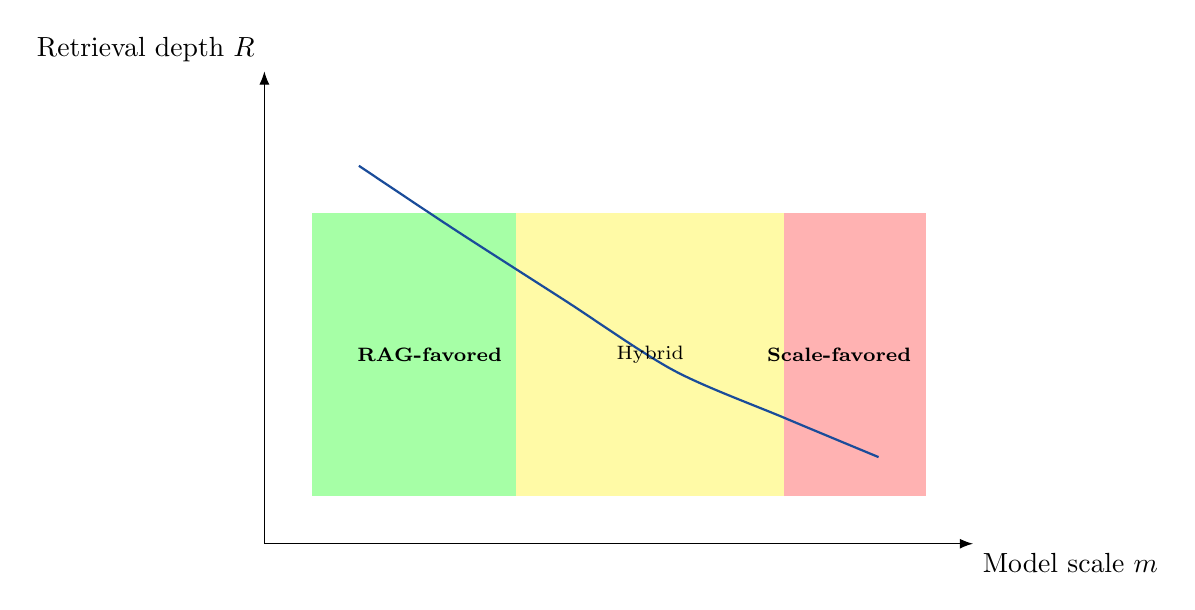
\begin{tikzpicture}[x=1cm,y=1cm,>=Latex]
  % axes
  \draw[->] (0,0) -- (9,0) node[below right]{Model scale $m$};
  \draw[->] (0,0) -- (0,6) node[above left]{Retrieval depth $R$};
  % regions (stylized)
  \fill[green!35] (0.6,0.6) rectangle (3.2,4.2);
  \fill[yellow!35] (3.2,0.6) rectangle (6.6,4.2);
  \fill[red!30] (6.6,0.6) rectangle (8.4,4.2);
  % efficient locus
  \draw[thick,linkblue,smooth] plot coordinates {(1.2,4.8) (2.4,4.0) (3.8,3.1) (5.2,2.2) (6.6,1.6) (7.8,1.1)};
  \node at (2.1,2.4) {\scriptsize \textbf{RAG-favored}};
  \node at (4.9,2.4) {\scriptsize Hybrid};
  \node at (7.3,2.4) {\scriptsize \textbf{Scale-favored}};
\end{tikzpicture}
\caption{RAG–scale efficiency map. The efficient locus equates marginal QOU-per-dollar; its position depends on $(\zeta_m,\zeta_R)$ and relative costs $(MC_m,MC_R)$.}
\label{fig:ragscale}
\end{figure}

% ================= 6. Implementation Protocol =================
\section{Implementation Protocol: Data and Reproducibility}
\paragraph{Data primitives.}
The measurement pipeline requires the following minimal tables, each row versioned with collection date and source metadata.

\begin{table}[H]
\centering
\begin{threeparttable}
\caption{Required data primitives and units}
\label{tab:primitives}
\begin{tabular}{l l l l}
\toprule
Table & Key fields & Units & Purpose \\
\midrule
Energy prices & region, date, $c_E$ & \si{\cent\per\kilo\watt\hour} & Factor price \\
Accelerator prices & SKU, region, date, \$/hr & \si{\dollar\per\hour} & GPU/instance cost \\
Network metrics & region$\to$region, p95 RTT & \si{\milliSecond} & Latency bounds \\
Benchmarks & task family, item id, score & unitless (0--1) & Accuracy $a$ \\
Reliability & service window, availability & fraction (0--1) & $q$ \\
Safety & audit pass share & fraction (0--1) & $s$ \\
\bottomrule
\end{tabular}
\begin{tablenotes}[flushleft]
\item \emph{Note:} Values are placeholders; in practice fill from (i) serving telemetry (utilization, p95 latency, batch sizes), (ii) benchmark panels mapping $(m,R,Z)$ to accuracy, and (iii) location-specific factor prices (energy tariffs, accelerator lease rates, RTTs).
\end{tablenotes}
\end{threeparttable}
\end{table}

\paragraph{Computation.}
(i) Normalize benchmark instances to task units at QoS thresholds; (ii) calibrate $(\eta_a,\eta_\ell,\eta_q,\eta_s)$ from revealed-preference or declared weights; (iii) estimate $(\zeta_m,\zeta_R,\theta_{\cdot})$ from panel regressions of benchmark scores on $(m,R,Z)$; (iv) map utilization to p95 latency using the serving model; (v) solve the convex surrogate of \eqref{eq:program} to obtain $c_{\mathcal T}$ and compute $\LCI$.

% ---- Table: Stylized calibration example ----
\begin{table}[t]
\centering
\begin{threeparttable}
\caption{Stylized calibration snapshot (illustrative)}
\label{tab:calib}
\begin{tabular}{l c c c c}
\toprule
Parameter & Value & SE & Source & Notes \\
\midrule
$\eta_a$ & 1.20 & (0.05) & RP weights & Accuracy elasticity \\
$\eta_\ell$ & 0.80 & (0.06) & SLA penalties & Latency penalty exponent \\
$\eta_q$ & 0.50 & (0.04) & Uptime SLAs & Reliability weight \\
$\eta_s$ & 0.40 & (0.03) & Audit logs & Safety weight \\
$\zeta_m$ & 0.35 & (0.02) & Scaling panel & Model scale exponent \\
$\zeta_R$ & 0.28 & (0.03) & Retrieval panel & Retrieval exponent \\
$\gamma$ & 1.60 & (0.10) & Ops telemetry & Congestion curvature \\
$u_{\max}$ & 0.92 & -- & Capacity plan & Saturation bound \\
\bottomrule
\end{tabular}
\begin{tablenotes}[flushleft]
\item \emph{Note:} Values are placeholders for illustration; replace with empirical estimates derived from (i) proprietary serving telemetry, (ii) benchmark panels, and (iii) location-specific factor price data.
\end{tablenotes}
\end{threeparttable}
\end{table}

% ================= 7. Intelligence Price Deflator =================
\section{Aggregation: The Intelligence Price Deflator (IPD)}
Let $\{\mathcal T_k\}$ denote task families with expenditure shares $s_{k,t}$ at time $t$. The national LCI index is a chain Fisher across families:
\begin{equation}
\IPD_t
= \prod_{\tau=1}^{t}\sqrt{
\sum_k s_{k,\tau-1}\,\frac{\LCI_{k,\tau}}{\LCI_{k,\tau-1}}
\cdot
\sum_k s_{k,\tau}\,\frac{\LCI_{k,\tau}}{\LCI_{k,\tau-1}}
}.
\end{equation}
Paasche/Laspeyres bounds follow. Decompositions separate within-family LCI changes, between-family share shifts, and entry/exit.

% ---- Figure: IPD example path ----
\begin{figure}[t]
\centering
\begin{tikzpicture}[x=0.8cm,y=0.08cm,>=Latex]
  % Axes
  \draw[->] (0,0) -- (14,0) node[below right]{Time (quarters)};
  \draw[->] (0,0) -- (0,120) node[above left]{Index (base=100)};
  % IPD path (stylized)
  \draw[thick,linkblue] plot coordinates {(1,100) (2,97) (3,95) (4,92) (5,90) (6,88) (7,86) (8,85) (9,84) (10,83) (11,82) (12,81) (13,80)};
  \node[linkblue] at (11,88) {\scriptsize IPD ($\downarrow$ = cheaper intelligence)};
  % Bounds
  \draw[dashed,gray] plot coordinates {(1,102) (2,99) (3,96) (4,94) (5,92) (6,90) (7,88) (8,87) (9,86) (10,85) (11,84) (12,83) (13,82)};
  \draw[dashed,gray] plot coordinates {(1,98) (2,95) (3,94) (4,90) (5,88) (6,86) (7,84) (8,83) (9,82) (10,81) (11,80) (12,79) (13,78)};
  \node[gray] at (4.5,102) {\scriptsize Laspeyres};
  \node[gray] at (4.5,94) {\scriptsize Paasche};
\end{tikzpicture}
\caption{Illustrative IPD trajectory with Laspeyres and Paasche bounds. Values are stylized for exposition.}
\label{fig:ipd}
\end{figure}

% ================= 8. Limitations =================
\section{Scope and Limitations}
LCI is a supply-side cost frontier. It does not incorporate demand elasticities or market power. QoS weights are policy or application parameters and must be predeclared. Multi-tenancy is costed via capacity reservations. Dependencies among QoS margins are handled conservatively by Bonferroni or CVaR surrogates. Real systems include multi-stage pipelines, heterogeneous pools, and dynamic load balancing; empirical mapping from utilization to p95 latency should be validated against telemetry.

% ================= 9. Conclusion =================
\section{Conclusion}
LCI prices what matters operationally: the cost per unit of usable intelligence at stated QoS. With a serving-aware model class, tractable chance constraints, and a clear aggregation procedure (IPD), the framework enables reproducible, location-aware measurement and supports architecture and infrastructure comparisons.
\par\medskip\noindent\textbf{Future research.} Two directions are immediate. First, integrate demand-side behavior (elasticities, pass-through, adoption frictions) to connect LCI to equilibrium PUI and welfare. Second, generalize the measurement object beyond discrete benchmarks to multi-step or continuous AI production processes (e.g., agentic workflows), incorporating inter-stage dependencies and pipeline-level QoS. Identification using natural experiments in energy prices, capacity shocks, or network upgrades can sharpen causal inference on the drivers of $\LCI$.

% ================= References =================
\begin{thebibliography}{}
\bibitem[Byrne and Syverson(2017)]{Byrne2017}
Byrne, D.\ M., and C.\ Syverson. 2017. ``Prices of Computing and Communication Equipment.'' \emph{American Economic Review} 107(5): 168--172.

\bibitem[Pakes(2003)]{Pakes2003}
Pakes, A. 2003. ``A Reconsideration of Hedonic Price Indexes with an Application to PCs.'' \emph{American Economic Review} 93(5): 1578--1596.

\bibitem[Triplett(1989)]{Triplett1989}
Triplett, J.\ E. 1989. ``Price Indexes for Military Electronics: A Hedonic Approach.'' \emph{Brookings Papers on Economic Activity, Microeconomics}: 373--438.
\end{thebibliography}

% ================= Appendices =================
\appendix

\section{Tractable Chance Constraints}\label{app:chance}
The joint constraint
\(
\PP(a\ge\bar a,\,\ell\le\bar\ell,\,q\ge\bar q,\,s\ge\bar s)\ge 1-\varepsilon
\)
is generally non-convex. We adopt either:

\paragraph{Bonferroni.}
Pick $(\varepsilon_a,\varepsilon_\ell,\varepsilon_q,\varepsilon_s)$ such that $\sum\varepsilon_i\le\varepsilon$, and enforce the marginal constraints separately. Each constraint is convex under standard distributional assumptions (e.g., affine uncertainty sets or moment bounds).

\paragraph{CVaR.}
Let $L\ge0$ be an economic loss that is zero when all QoS thresholds hold and positive otherwise (e.g., a weighted hinge). Enforce $\mathrm{CVaR}_{\varepsilon}(L)\le 0$. This is convex in decision variables whenever $L$ is convex.

\section{Queueing-Theoretic Basis for Property C}\label{app:queue}
Assume (i) GI/G/$k$ with processor sharing and micro-batching $(B,\tau_b)$; (ii) finite second moments for inter-arrival and service times; (iii) many-server heavy traffic ($k\to\infty$ with $(1-u)\sqrt{k}\to\beta$). In this Halfin–Whitt regime, diffusion approximations imply convexity of high-quantile response times in $u$ on $[u_0,u_{\max})$ for some $u_0<1$. Because $\partial \QOU/\partial \ell<0$ and $\lambda(\ell)$ is smooth and strictly decreasing for $\ell>\bar\ell$, $\LCI(u)$ inherits convexity near saturation. Micro-batching rescales effective service and inflates variability; under bounded moments, convexity of $W_{0.95}(u)$ is preserved.

\section{Empirical Protocol and Reproducible Artifacts}\label{app:empirical}
\paragraph{Data release.}
Provide CSVs for primitives (Table~\ref{tab:primitives}), a JSON schema for QoS thresholds, and a configuration file for location prices. Include a notebook that (i) estimates parameters in Table~\ref{tab:calib}, (ii) validates the mapping $u\mapsto W_{0.95}(u)$, and (iii) recomputes $\LCI$ and $\IPD$.

\paragraph{Versioning.}
Each run stores Git commit hash, data snapshot time, and solver settings. Outputs include $\LCI$ by task family, location comparisons, and uncertainty bands via bootstrap.

\end{document}
